% ======================================================================
% LAST MODIFICATION ON (MONTH / DAY / YEAR): 7/27/20
% ======================================================================
\documentclass[12pt, % tamanho da fonte
               openright, % capítulos começam em pág ímpar
                          % (insere página vazia caso preciso)
               oneside, % para impressão apenas em um lado do papel
               a4paper, % tamanho do papel.
               chapter=TITLE, % títulos de capítulos convertidos em
                              % letras maiúsculas
               section=TITLE, % títulos de seções convertidos em letras
                              % maiúsculas
               % subsection=TITLE, % títulos de subseções convertidos em
                                 % letras maiúsculas
               % subsubsection=TITLE, % títulos de subsubseções em letras
                                    % maiúsculas
               % sumario=tradicional,
               brazil,
               english % o último idioma é o principal do documento
]{abntex2}
% ----------------------------------------------------------------------
% \renewcommand{\ABNTEXsectionfont}{\normalfont}
\renewcommand{\cftsectionfont}{\normalsize}
% ----------------------------------------------------------------------
\renewcommand{\ABNTEXchapterfontsize}{\bfseries\large}
\renewcommand{\ABNTEXsectionfontsize}{\large}
\renewcommand{\ABNTEXsubsectionfontsize}{\large}
% ----------------------------------------------------------------------
\usepackage{lastpage}
% \usepackage{times}
\usepackage{etoolbox}
\usepackage{lmodern} % usa a fonte Latin Modern
% \usepackage[T1]{fontenc} % selecao de codigos de fonte
\usepackage[utf8]{inputenc} % sodificacao do documento (conversão
                            % automática dos acentos)
% \usepackage{lastpage} % ssado pela ficha catalográfica
\usepackage{indentfirst} % indenta o primeiro parágrafo de cada seção
\setlength{\parindent}{1.5cm} % espaçamento de 1.5cm do parágrafo
\usepackage{color} % controle das cores
\usepackage{graphicx} % inclusão de gráficos
\usepackage{microtype} % para melhorias de justificação
\usepackage{setspace}
\usepackage{pdflscape} % pagina na horizontal
% \usepackage{lscape} % pagina na horizontal
\usepackage{wrapfig}
\usepackage{pgf} % para geração de dummy text
\usepackage[english, hyperpageref]{backref} % paginas com as citações
% ----------------------------------------------------------------------
% quadro cinza =========================================================
% \usepackage{caption}
\usepackage[small]{caption}
\usepackage{tikz} % permite desenhos vetoriais
% define o ambiente para colocar o código R
% (draw=gray!50 fill=gray!20 originais)
\tikzstyle{mybox} = [draw=gray!95, fill=white, very thick, rectangle,
                     inner sep=7pt, inner ysep=7pt]
\tikzstyle{mybox2} = [draw=gray!50, fill=gray!20,
                      very thick, % para códigos em R (Apêndices)
                      rectangle, inner sep=7pt, inner ysep=7pt]
% \usepackage[scaled=0.8]{beramono} % usa esta nos verbatins
\usepackage{float} % controla e define objetos flutuantes
\usepackage{tocloft} % controla lista de objetos flutuantes
% ambiente flutuante para código R
\newcommand{\listofprogramname}{CODE} % nome dessa lista
\newlistof{program}{lol}{\listofprogramname} % configura os arquivos
                                             % auxiliares para fazer a
                                             % lista
\makeatletter % allows use of "@" before \begin{document}
% this creates a custom and simpler ruled box style
\newcommand\floatc@simplerule[2]{{\@fs@cfont #1 #2}\par}
\newcommand\fs@simplerule{\def\@fs@cfont{ % aqui o estilo de fonte, e.g.
                                          % \bfseries
  }\let\@fs@capt\floatc@simplerule
  \def\@fs@pre{} % antes do caption, pode ser uma régua
  \def\@fs@post{} % depois do float, pode ser uma régua
  \def\@fs@mid{\kern3pt} % espaço entre caption e corpo
  \let\@fs@iftopcapt\iftrue}
\floatstyle{simplerule} % define o estilo do ambiente
\newfloat{program}{thp}{lol}[chapter] % ambiente contado por capítulo
\floatname{program}{Code} % rótulo que vai aparecer na legenda
\newcommand{\programautorefname}{Code} % altera o padrão do contador
                                       % para seguir capítulos
\renewcommand{\theprogram}{\thechapter.\arabic{program}} % capítulo.
                                                         % programa:
\sloppy
% FIM - TIKZ (quadro cinza) ============================================
% ----------------------------------------------------------------------
% CONFIGURAÇÕES DE PACOTES
% Configurações do pacote backref
% Usado sem a opção hyperpageref de backref
\renewcommand{\backrefpagesname}{Cited in the page(s):~}
% Texto padrão antes do número das páginas
\renewcommand{\backref}{}
% Define os textos da citação
\renewcommand*{\backrefalt}[4]{
  \ifcase #1 %
  None text citation.%
  \or
  Cited on page #2.%
  \else
  Cited #1 times on pages #2.%
  \fi}%
% ----------------------------------------------------------------------
\usepackage[alf]{abntex2cite}	% Citações padrão ABNT
% ----------------------------------------------------------------------
% New comand for anexos
\newcommand{\refanexo}[1]{\hyperref[#1]{Annex~\ref{#1}}}
% \renewcommand{\cftsectionfont}{\sfseries}
% \refanexo{anexo_xxx} usar esse comando!
% ----------------------------------------------------------------------
% para titulo em destaque sem sequencia de numeração
\newcommand{\datatitle}[1]{
  \normalsize \textsc{#1}
}
\usepackage{pslatex}
% \usepackage{mathptmx} fonte - times new roman em tudo
% ----------------------------------------------------------------------
% adequando o uppercase titulo dos elementos nas suas respectivas LISTAS
\renewcommand{\cftfigurename}{FIGURE\enspace}
\renewcommand{\cfttablename}{TABLE\enspace}
% ----------------------------------------------------------------------
% fontes matemáticas
\usepackage{mathpazo}
\usepackage{inconsolata}
\usepackage{verbatim}
% ----------------------------------------------------------------------
% \usepackage[table, xcdraw]{xcolor} % cédula colorida em tabelas
% \usepackage{pdflscape} % rotaciona página
\usepackage{Capa} % capa e folha de rosto com modificações
\usepackage{float} % melhor posicionamento de figuras
\usepackage{gensymb} % símbolo º
\usepackage[justification=justified, singlelinecheck=false]{caption}
% \usepackage{etoolbox} % configurações adicionais de macros
\usepackage{xparse}
\usepackage{algorithm} % pacote usado para gerar pseudocódigo
\usepackage{algorithmic} % pacote usado para gerar pseudocódigo
\usepackage{listings}
\usepackage{multirow}
% ----------------------------------------------------------------------
% pacote para fazer o checkmark
\usepackage{pifont} % http://ctan.org/pkg/pifont
\newcommand{\cmark}{\ding{51}}%
\newcommand{\xmark}{\ding{55}}%
% ----------------------------------------------------------------------
\usepackage{amsmath}
\usepackage{amsfonts}
\usepackage{amssymb}
\usepackage{pdfpages}
% \usepackage{times}
% \usepackage{helvet}
% \renewcommand{\familydefault}{\sfdefault}
% ----------------------------------------------------------------------
\NewDocumentCommand\cc{+u{\cc}}{\ignorespaces}
% ----------------------------------------------------------------------
% controle do espaçamento entre um parágrafo e outro:
\setlength{\parskip}{0.2cm} % tente também \onelineskip
% ----------------------------------------------------------------------
\titulo{A MULTINOMIAL GLMM FOR COMPETING RISK DATA}
\autor{HENRIQUE APARECIDO LAUREANO}
\data{2020}
\instituicao{FEDERAL UNIVERSITY OF PARANÁ}
\orientador{Prof. PhD Wagner Hugo Bonat}
\coorientador{Prof. PhD Paulo Justiniano Ribeiro Jr}
\tipotrabalho{Dissertação (mestrado)}
\preambulo{\small{Thesis presented to the Graduate Program of Numerical
    Methods in Engineering, Concentration Area in Mathematical
    Programming: Statistical Methods Applied in Engineering, Federal
    University of Paran\'{a}, as part of the requirements to the
    obtention of the Master's Degree in Sciences.}}
% ----------------------------------------------------------------------
% informações do PDF
\makeatletter
\hypersetup{
  % pagebackref=true,
  pdftitle={\@title},
  pdfauthor={\@author},
  pdfsubject={\imprimirpreambulo},
  % pdfkeywords = {}{}{}{},
  colorlinks=true, % false: boxed links; true: colored links
  linkcolor=blue, % color of internal links
  citecolor=blue, % color of links to bibliography
  filecolor=magenta, % color of file links
  urlcolor=blue,
  bookmarksdepth=4
}
\addto\captionsenglish{
  % adjusts names from abnTeX2
  \renewcommand{\folhaderostoname}{Title page}
  \renewcommand{\epigraphname}{Epigraph}
  \renewcommand{\dedicatorianame}{Dedication}
  \renewcommand{\errataname}{Errata sheet}
  \renewcommand{\agradecimentosname}{Acknowledgements}
  \renewcommand{\anexoname}{ANNEX}
  \renewcommand{\anexosname}{Annex}
  \renewcommand{\apendicename}{APPENDIX}
  \renewcommand{\apendicesname}{Appendix}
  \renewcommand{\orientadorname}{Supervisor:}
  \renewcommand{\coorientadorname}{Co-supervisor:}
  \renewcommand{\folhadeaprovacaoname}{Approval}
  \renewcommand{\resumoname}{Abstract}
  \renewcommand{\listadesiglasname}{List of abbreviations and acronyms}
  \renewcommand{\listadesimbolosname}{List of symbols}
  \renewcommand{\fontename}{Source}
  \renewcommand{\notaname}{Note}
  % adjusts names used by \autoref
  \renewcommand{\pageautorefname}{page}
  \renewcommand{\sectionautorefname}{section}
  \renewcommand{\subsectionautorefname}{subsection}
  \renewcommand{\subsubsectionautorefname}{subsubsection}
  \renewcommand{\paragraphautorefname}{subsubsubsection}
}
\makeatother
% ----------------------------------------------------------------------
\graphicspath{{Figuras/}}
% ----------------------------------------------------------------------
\begin{document}
\selectlanguage{english}
% adequando o uppercase titulo dos elementos nas suas respectivas
% legendas
\renewcommand{\tablename}{TABLE }
\renewcommand{\figurename}{FIGURE }
% ----------------------------------------------------------------------
\frenchspacing % retira espaço extra obsoleto entre as frases
% ----------------------------------------------------------------------
% capa
\tikz[remember picture,overlay] \node[opacity=1,inner sep=0pt] at
(current page.center){
  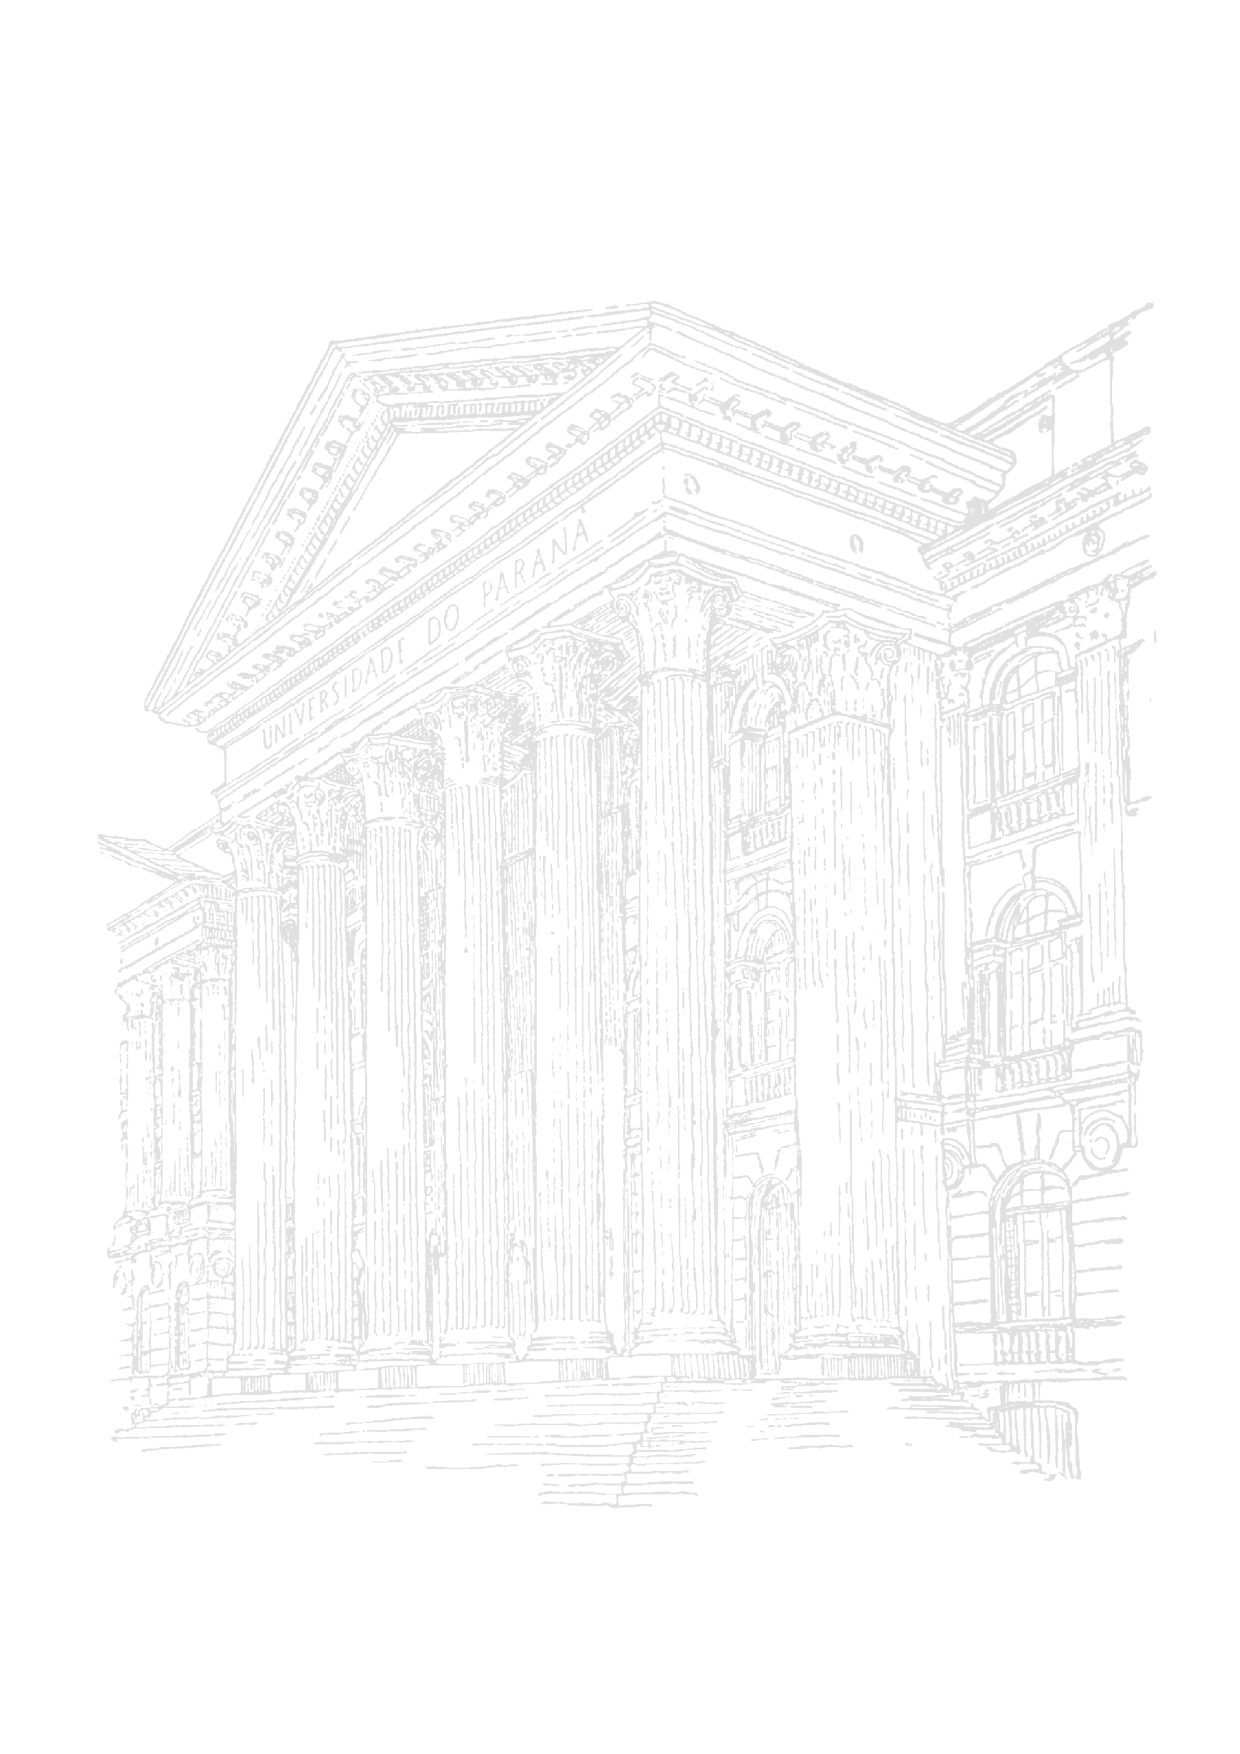
\includegraphics[width=\paperwidth,
  height=\paperheight]{Figuras/ufpr_bg}};
% ----------------------------------------------------------------------
\imprimircapa
% ----------------------------------------------------------------------
% folha de rosto
\imprimirfolhaderosto
% ----------------------------------------------------------------------

% \begin{dedicatoria}
%   \vspace*{\fill}
%   ...
%   \vspace*{\fill}
% \end{dedicatoria}
% ----------------------------------------------------------------------
% ficha catalográfica

% \begin{fichacatalografica}
%   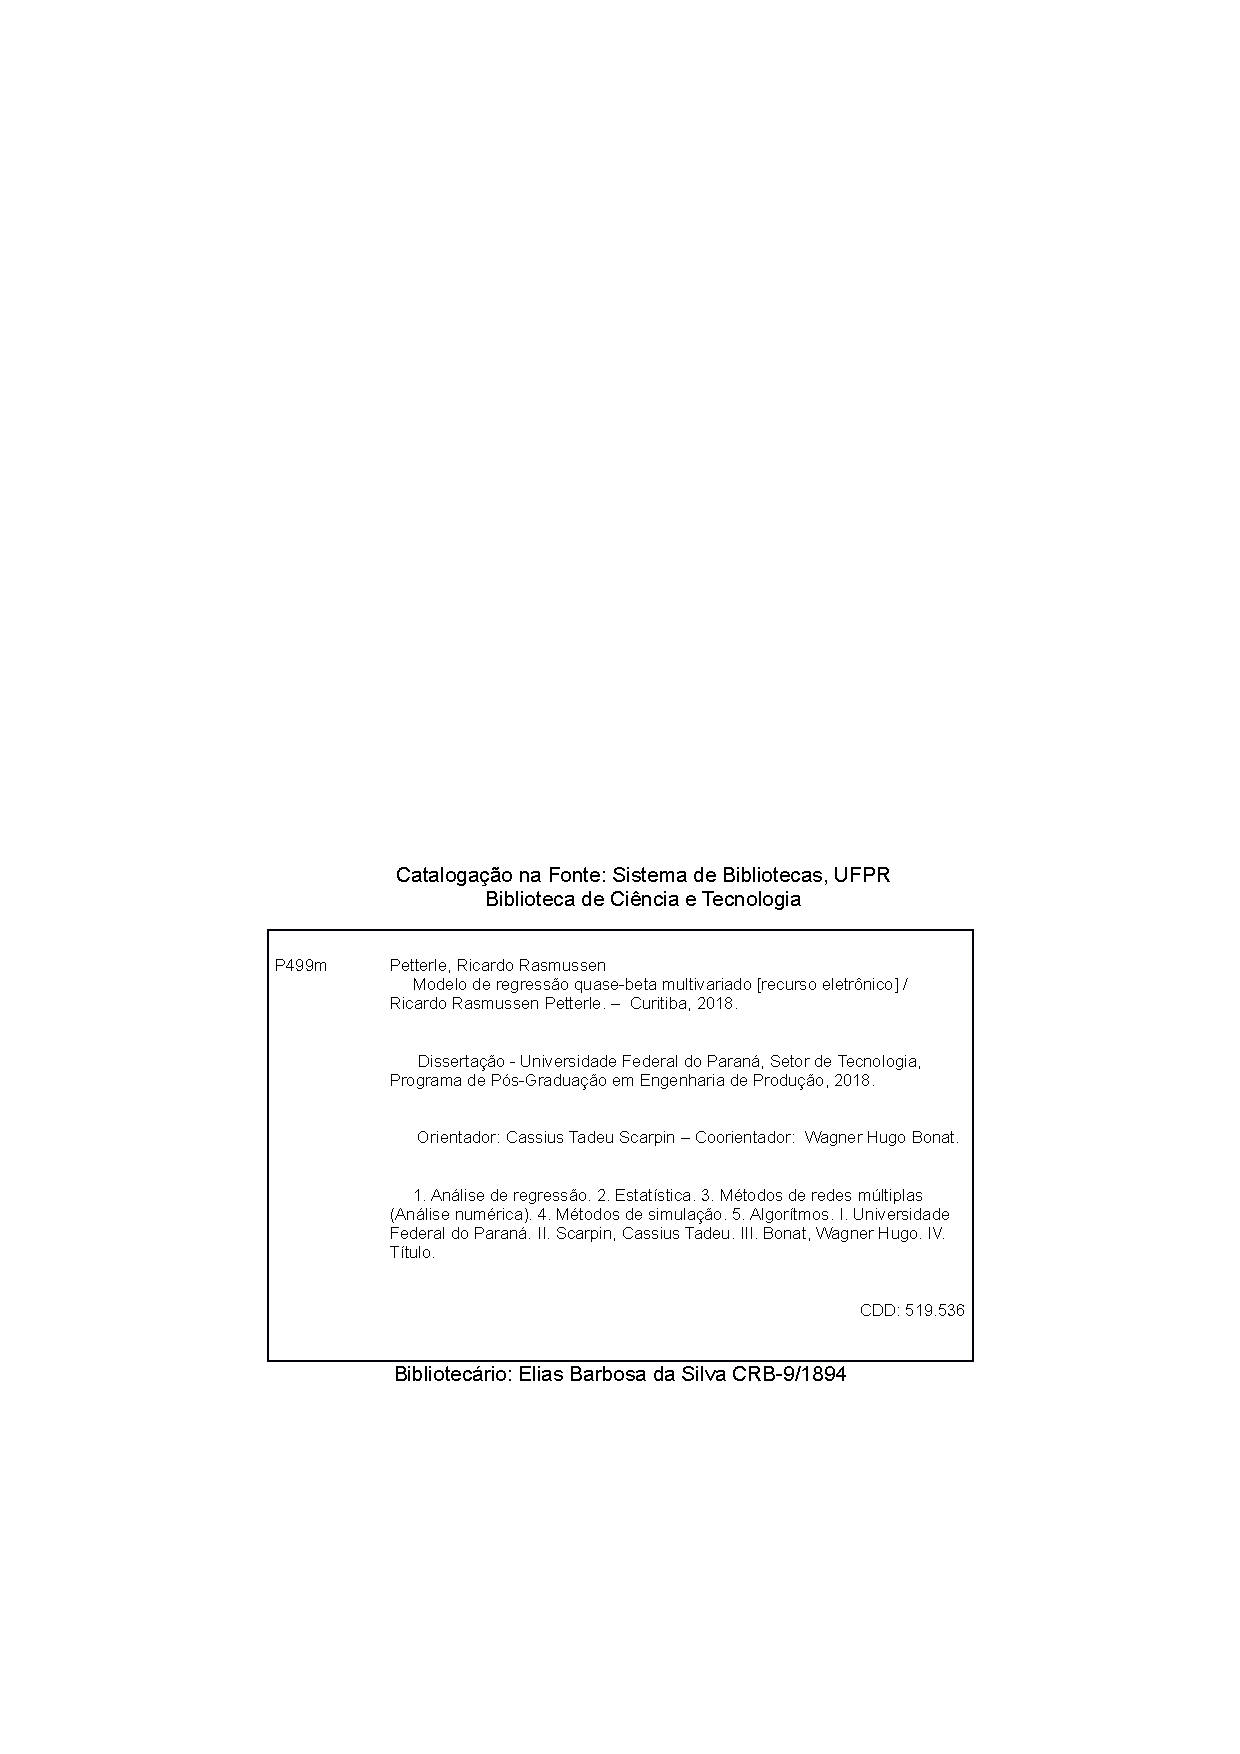
\includepdf{ficha.pdf}
% \end{fichacatalografica}
% ----------------------------------------------------------------------
% inserir folha de aprovação
% \begin{folhadeaprovacao}
%   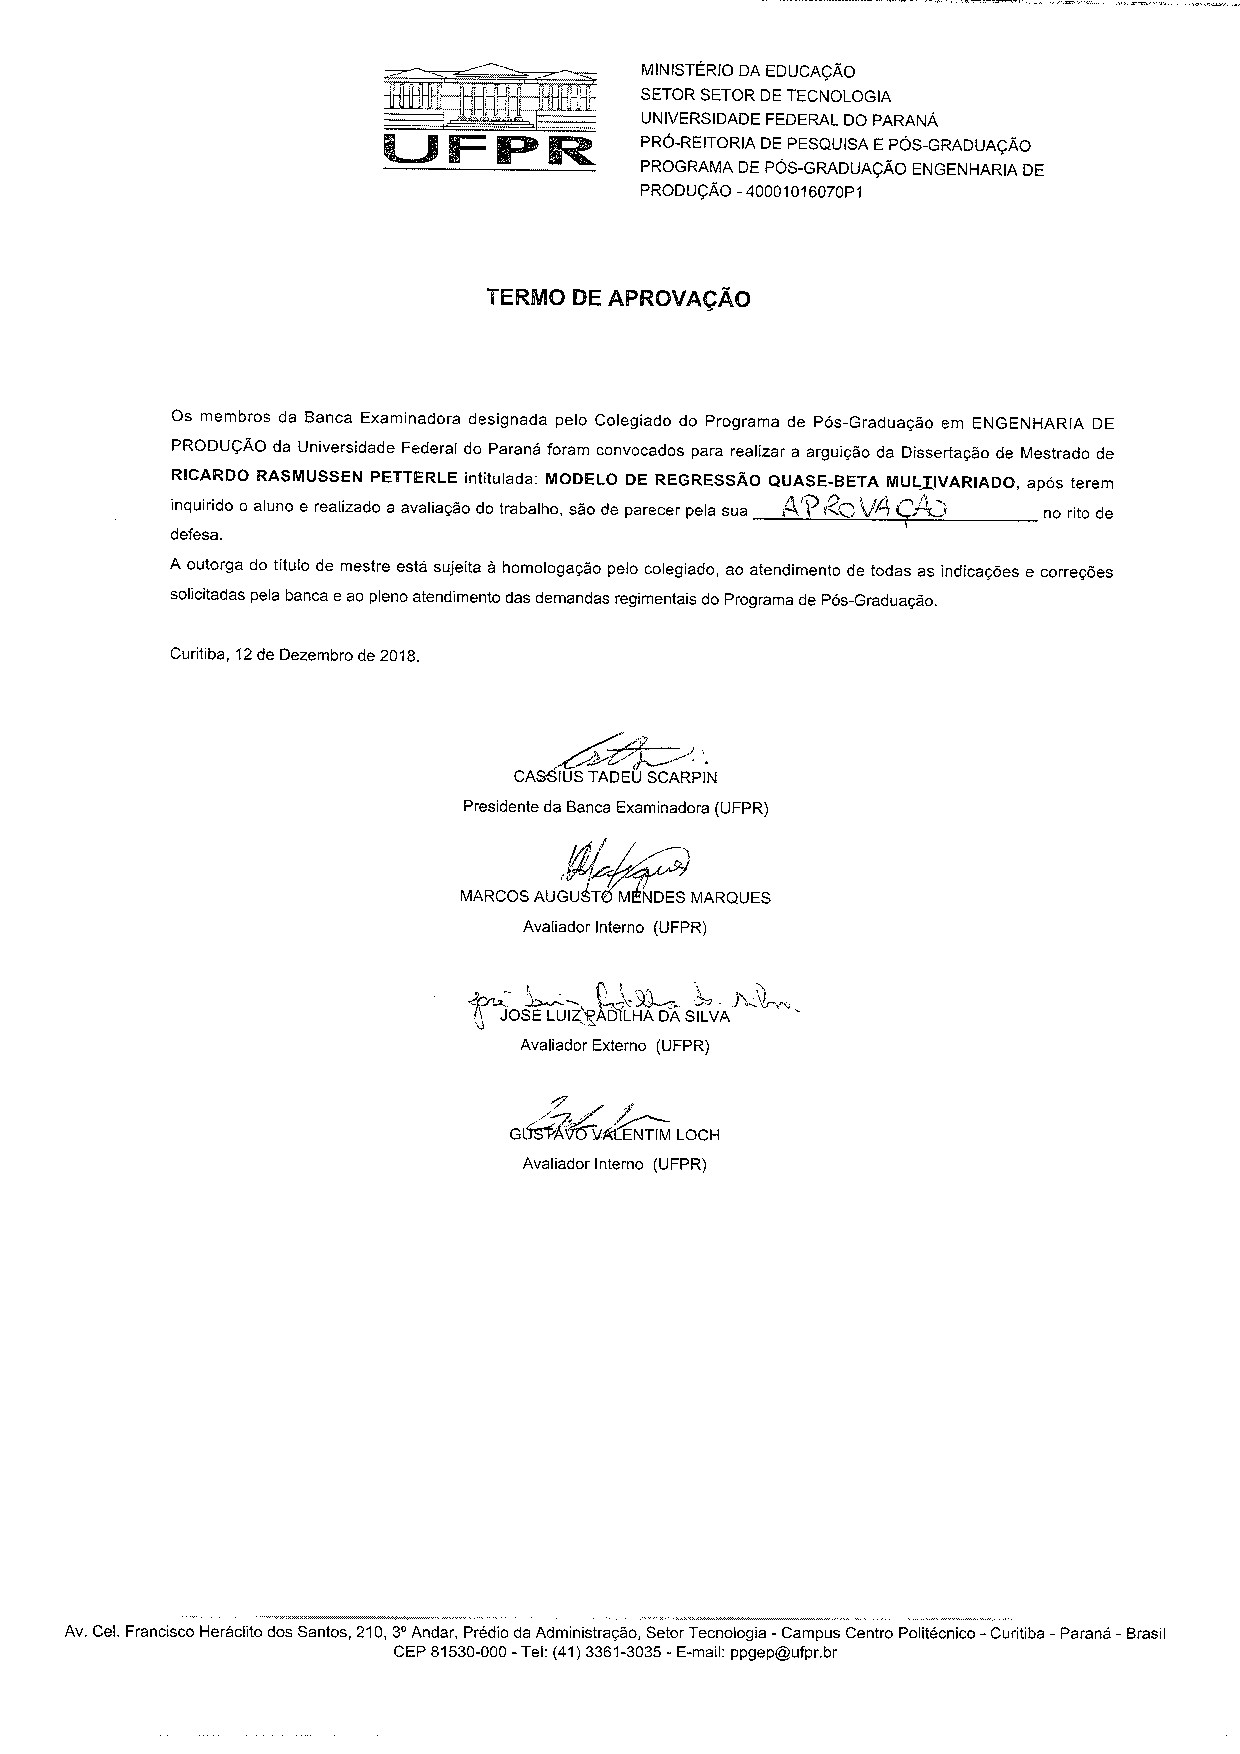
\includepdf{termo.pdf}
% \end{folhadeaprovacao}
\begin{folhadeaprovacao}
 \begin{center}
   {\ABNTEXchapterfont\large\imprimirautor}

   \vspace*{\fill}\vspace*{\fill}
   \begin{center}
     \ABNTEXchapterfont\bfseries\large\imprimirtitulo
   \end{center}
   \vspace*{\fill}

    \hspace{.45\textwidth}
    \begin{minipage}{.5\textwidth}
       \imprimirpreambulo
    \end{minipage}
   \vspace*{\fill}
 \end{center}

 Master thesis approved. XXX XX, 2020.

  \assinatura{\textbf{\imprimirorientador} \\ Supervisor}
  \assinatura{\textbf{Prof. PhD Paulo Justiniano Ribeiro Jr} \\
    Co-supervisor}
  \assinatura{\textbf{Prof. PhD ...} \\Internal Examinator - PPGMNE}
  \assinatura{\textbf{Prof. PhD ...} \\Internal Examinator - PPGMNE}
  \assinatura{\textbf{Prof. PhD ...} \\External Examiner - }

  \begin{center}
   \vspace*{0.5cm}
   {\large CURITIBA}
   \par
   {\large\imprimirdata}
   \vspace*{1cm}
 \end{center}

\end{folhadeaprovacao}
% ----------------------------------------------------------------------
\begin{dedicatoria}
  \vspace*{22.7cm}
  \begin{flushright}
    \begin{minipage}[H]{4.5cm}
      {To Celita and Olivio}
    \end{minipage}
  \end{flushright}
\end{dedicatoria}
% ----------------------------------------------------------------------
\begin{agradecimentos}
  ...
\end{agradecimentos}

\begin{epigrafe}
  \vspace*{\fill}
  \begin{flushright}
    \textit{"A simplicidade é o último grau de sofisticação".\\
      (Leonardo da Vinci)}
  \end{flushright}
\end{epigrafe}
% ----------------------------------------------------------------------
\newpage
\setlength{\absparsep}{18pt} % ajusta o espaçamento dos parágrafos do
                             % resumo
\setlength{\abstitleskip}{1cm} % adiciona mais um cm após o 'titulo' do
                               % resumo para ficar com 2cm
\begin{resumo}[]
  \vspace{-2cm}
  \begin{center}
    \bfseries{\large{\textsf{ABSTRACT}}}
  \end{center}
  \vspace{0.3cm}
  ...

  \textbf{Keywords}: . . . . . .
\end{resumo}
% ----------------------------------------------------------------------
\newpage
\setlength{\absparsep}{18pt} % ajusta o espaçamento dos parágrafos do
                             % resumo
\setlength{\abstitleskip}{1cm} % adiciona mais um cm após o 'titulo' do
                               % resumo para ficar com 2cm
\begin{resumo}[]
  \begin{otherlanguage*}{brazil}
    \vspace{-2cm}
    \begin{center}
      \bfseries{\large{\textsf{RESUMO}}}
    \end{center}
    \vspace{0.3cm}
    ...

    \textbf{Palavras-chave}: . . . . . .
  \end{otherlanguage*}
\end{resumo}
% ----------------------------------------------------------------------
\pdfbookmark[0]{\listfigurename}{lof}
\listoffigures*
\cleardoublepage
% ----------------------------------------------------------------------
\pdfbookmark[0]{\listtablename}{lot}
\listoftables*
\cleardoublepage
% ----------------------------------------------------------------------
% \begin{siglas}
% \item[Fig.] Area of the $i^{th}$ component
% \item[456] Isto éum número
% \item[123] Isto éoutro número
% \item[lauro cesar] este éo meu nome
% \end{siglas}
% ----------------------------------------------------------------------
\pdfbookmark[0]{\contentsname}{toc}
\tableofcontents*
\cleardoublepage
% ----------------------------------------------------------------------
\makepagestyle{abntheadings}
\makeevenhead{abntheadings}{\ABNTEXfontereduzida\thepage}{}{}
\makeoddhead{abntheadings}{}{}{\ABNTEXfontereduzida\thepage}
\makeheadrule{abntheadings}{\textwidth}{0in}
% ----------------------------------------------------------------------
\textual
% ----------------------------------------------------------------------
\chapter{Introdução}
\label{cap:introducao}
% ======================================================================

Em diversas áreas de pesquisa é comum investigar a relação entre uma
variável de interesse com outras variáveis que compõem o estudo. Para
tanto, faz-se uso da técnica estatística de modelos de regressão, uma
vez que se pode estudar o relacionamento entre uma variável
resposta~(variável dependente) com possíveis variáveis
explicativas~(covariáveis)~\cite{montgomery2012introduction}. A
aplicação desta técnica estatística é ampla, abrangendo diversas áreas
do conhecimento como medicina, engenharias, agronomia, ciências sociais
dentre outras. Nesse contexto, um dos principais modelos de regressão e
sem dúvida um dos mais usados por usuários de estatística aplicada é o
clássico modelo de regressão linear (Gaussiano). No entanto, para uso
desse modelo alguns pressupostos devem ser atendidos, tais como erros
independentes e identicamente distribuídos segundo a distribuição normal
com média zero e variância constante~\cite{draper2014applied}. Na
prática, isso nem sempre acontece e a má especificação desse modelo pode
gerar erros padrões inconsistentes, além de outros problemas que
invalidam todo o processo de
inferência~\cite{myersmontgomeryvining,montgomery2012introduction}.
Apesar de amplamente utilizado, o modelo de regressão linear não é
adequado para respostas binárias, politômicas, contagens ou limitadas.

% ----------------------------------------------------------------------
\section{OBJETIVOS}
% ----------------------------------------------------------------------

% ----------------------------------------------------------------------
\subsection{Objetivo geral}
% ----------------------------------------------------------------------

Propor um modelo de regressão para análise de variáveis respostas
limitadas multivariada.

% ----------------------------------------------------------------------
\subsection{Objetivos específicos}
% ----------------------------------------------------------------------

\begin{enumerate}
\item Estudar o desempenho do algoritmo NORTA (\emph{NORmal To
    Anything}) para simular variáveis aleatórias beta correlacionadas.

\item Especificar o modelo usando suposições de primeiro e segundo
  momentos.

\item Usar as funções de estimação quase-score e Pearson para estimar os
  parâmetros de regressão e dispersão, respectivamente.

\item Delinear estudos de simulação para explorar a flexibilidade do
  modelo para lidar com dados limitados em estudos longitudinais, além
  de checar propriedades dos estimadores em estudos com múltiplas
  respostas correlacionadas.

\item Adaptar técnicas de diagnóstico para o modelo proposto, como
  DFFITS, DFBETAS, distância de Cook e o gráfico de probabilidade
  meio-normal com envelope simulado.

\item Aplicar o modelo proposto em dois conjuntos de dados.
\end{enumerate}

% ----------------------------------------------------------------------
  \section{JUSTIFICATIVA}
% ----------------------------------------------------------------------

% ----------------------------------------------------------------------
\section{LIMITAÇÕES}
% ----------------------------------------------------------------------

Este trabalho se restringe a propor um novo modelo de regressão para
análise de variáveis respostas limitadas multivariada. Para motivar o
novo modelo, serão apresentadas aplicações em dois conjuntos de dados,
que não são facilmente manipulados pelos métodos estatísticos
existentes. Portanto, testes de hipóteses e de comparações múltiplas
multivariados não serão desenvolvidos no decorrer deste trabalho.

% ----------------------------------------------------------------------
\section{ORGANIZAÇÃO DO TRABALHO}
% ----------------------------------------------------------------------

Esta dissertação contém seis capítulos incluindo esta introdução.
O~\autoref{cap:aplicacoes} descreve os dois conjuntos de dados que serão
usados como exemplos de aplicação no novo modelo.
O~\autoref{cap:fundamentacaoteorica} apresenta a revisão bibliográfica
que motivou este trabalho, introduz o modelo de regressão beta
(univariado), apresenta o algoritmo NORTA (\textit{NORmal To Anything})
usado nos estudos de simulação e discute brevemente as medidas de
bondade de ajuste usadas no trabalho. O~\autoref{cap:multivariatemodel}
propõe o modelo de regressão quase-beta multivariado, apresenta o método
usado para estimação e inferência e adapta técnicas de diagnóstico.
No~\autoref{cap:resultados} são apresentados os resultados de três
estudos de simulação, além da análise dos dados apresentados
no~\autoref{cap:aplicacoes}. Finalmente, o~\autoref{cap:considefinais}
discute as principais contribuições desta dissertação, além de
apresentar as conclusões seguidas por sugestões para futuros trabalhos.

% END ==================================================================
% ----------------------------------------------------------------------
\chapter{Conjuntos de dados}
\label{cap:aplicacoes}
% ======================================================================

Este Capítulo descreve os dois conjuntos de dados que serão usados como
exemplos de aplicação no novo modelo de regressão, proposto no
\autoref{cap:multivariatemodel}. O primeiro conjunto se refere ao índice
de qualidade da água de reservatórios de usinas hidrelétricas operadas
pela COPEL no Estado do Paraná. Já o segundo conjunto de dados
corresponde ao percentual de gordura corporal de indivíduos avaliados no
Hospital de Clínicas da Universidade Federal do Paraná.

\section{CONJUNTO DE DADOS I: ÍNDICE DE QUALIDADE DA ÁGUA}
\label{cap:IQA}

\begin{table}[H]
  \centering
  \setlength{\abovecaptionskip}{.0001pt}
  \caption{ANÁLISE DESCRITIVA PARA O IQA POR TRIMESTRE E LOCAL}
  \label{tab:descIQA}
  \begin{tabular}{cccc}
    \hline
    \multirow{2}{*}{Trimestre} & \multicolumn{3}{c}{Local} \\
    \cline{2-4}  & Montante & Reservatório & Jusante \\
    \cline{2-4} 1   & $0,75\pm 0,11$   &  $0,80\pm 0,10$  &  $0,78\pm 0,10$  \\
    2  &  $0,79\pm 0,10$  &  $0,83\pm 0,06$   &  $0,83\pm 0,07$     \\
    3   &  $0,81\pm 0,07$   & $0,85\pm 0,05$   &  $0,83\pm 0,06$    \\
    4   & $0,76\pm 0,10$    &  $0,81\pm 0,08$    &  $0,79\pm 0,09$    \\
    \hline
  \end{tabular}
  \begin{footnotesize}
    \vspace{0.05cm}
    FONTE: O autor~(2018). \hspace{6.2cm}
    \vspace{-0.15cm}
  \end{footnotesize}
\end{table}

\vspace{-0.2cm}

\begin{figure}[H]
  \vspace{0.35cm}
  \setlength{\abovecaptionskip}{.0001pt}
  \caption{HISTOGRAMA~(A) E BOXPLOTS PARA O ÍNDICE DE QUALIDADE DA ÁGUA
    (IQA) POR TRIMESTRE~(B), LOCAL~(C) E USINAS~(D)}
  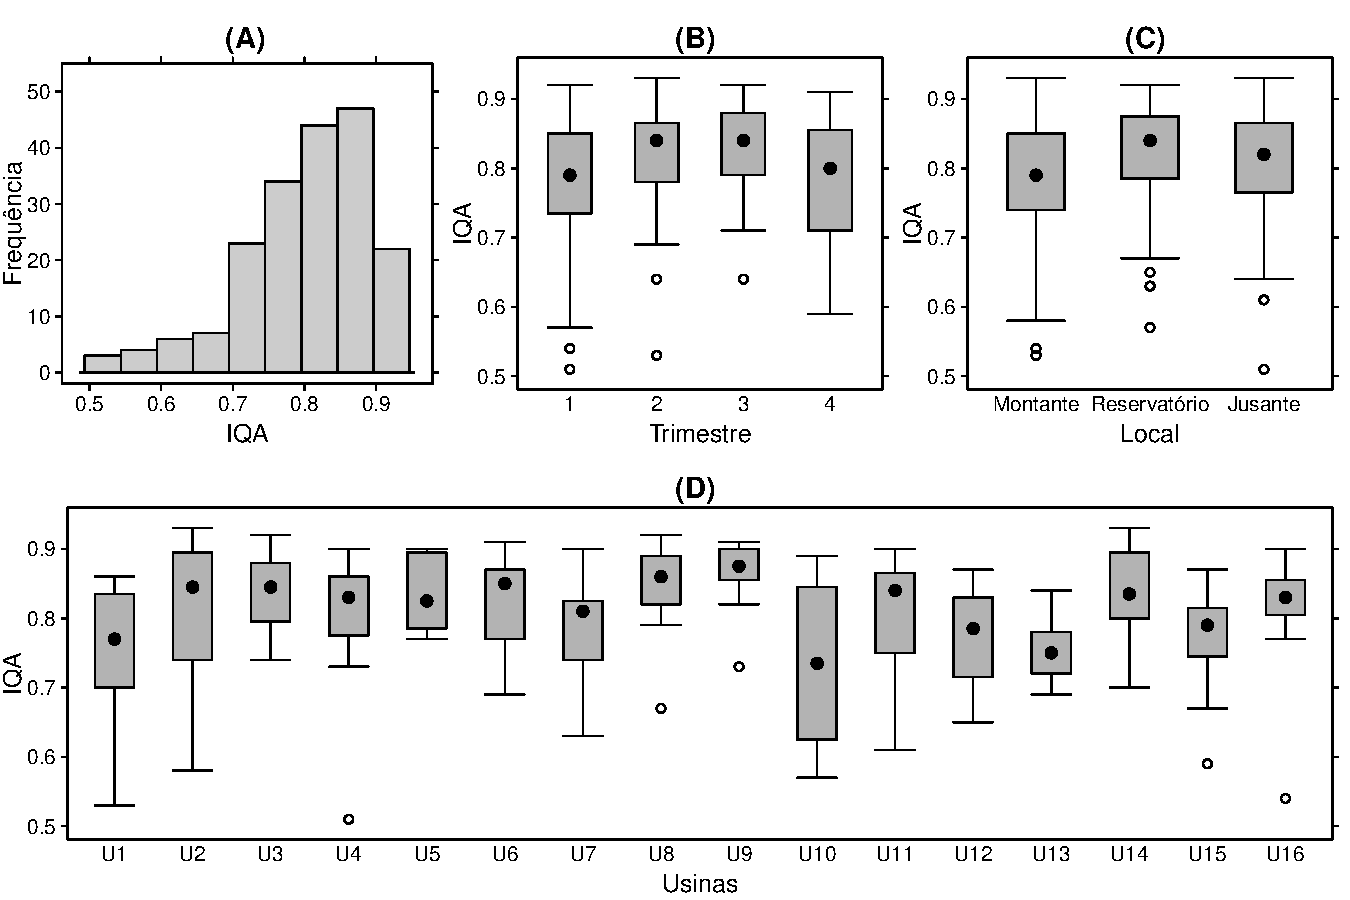
\includegraphics[width=0.95\textwidth]{Figure2.pdf}
  \begin{footnotesize}
    \vspace{-0.20cm}
    \centering
    FONTE: O autor~(2018).
    \vspace{0.15cm}
  \end{footnotesize}
  \label{fig:iqa1}
\end{figure}

Por fim, os resultados apresentados na~\autoref{fig:iqa1}~(D) mostram
que o IQA não é homogêneo entre as usinas, com um destaque maior para as
usinas 1, 2 e 10. É importante ressaltar que os resultados apresentados
na~\autoref{tab:descIQA} e~\autoref{fig:iqa1} se referem apenas a
análise descritiva e exploratória dos dados, onde são criadas hipóteses
que serão confirmadas somente após ajuste do modelo de regressão
proposto no~\autoref{cap:multivariatemodel}. No~\autoref{cap:apendiceA}
são apresentados gráficos boxplots para o IQA separado por trimestre e
local em função das usinas.

% ======================================================================
% ----------------------------------------------------------------------
\chapter{Fundamentação teórica}
\label{cap:fundamentacaoteorica}
% ======================================================================

Este Capítulo apresenta a fundamentação teórica que será usada nesta
dissertação. A~\autoref{cap:refteorico} apresenta um breve resumo dos
principais trabalhos relacionados ao assunto. A distribuição de
probabilidade beta e suas propriedades encontram-se
na~\autoref{cap:densbeta}. A~\autoref{cap:norta} apresenta o algoritmo
NORTA, que será usado para simular variáveis aleatórias beta
correlacionadas. A~\autoref{cap:betamodel} introduz o modelo de
regressão beta (univariado). Por fim, a~\autoref{cap:gof} apresenta
brevemente as medidas de bondade de ajuste usadas na comparação entre os
modelos.

\section{REVISÃO DA LITERATURA}
\label{cap:refteorico}

\section{DISTRIBUIÇÃO DE PROBABILIDADE BETA}
\label{cap:densbeta}

\begin{figure}[!htb]
  \centering
  \vspace{0.35cm}
  \setlength{\abovecaptionskip}{.0001pt}
  \caption{FUNÇÃO DE DISTRIBUIÇÃO BETA PARA DIFERENTES VALORES DE $\mu$
    COMBINADOS COM $\phi = (0,00001;~0,666;~4;~9;~23,99)$}
  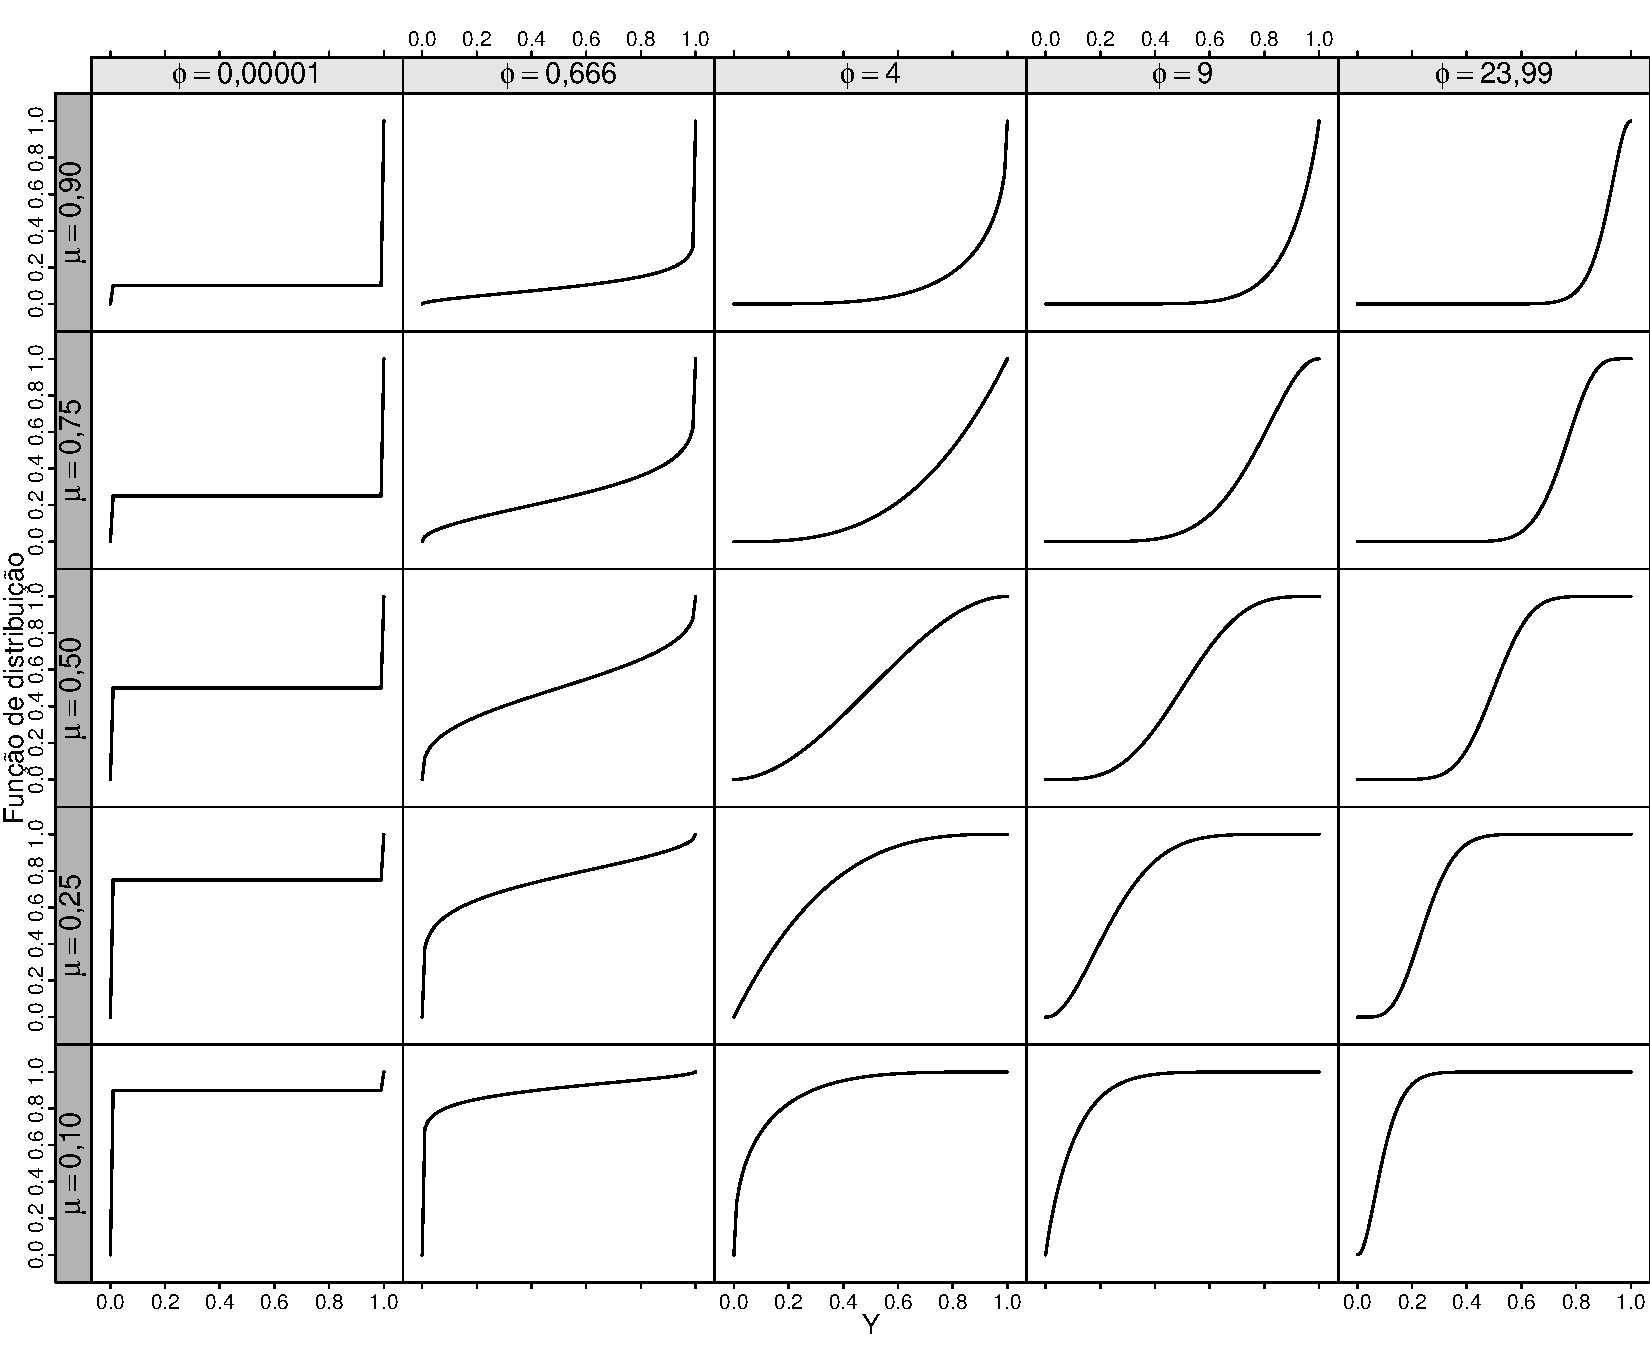
\includegraphics[width=.9\textwidth]{Figure6.pdf}
  \begin{footnotesize}
    \vspace{-0.1cm}
    FONTE: O autor~(2018).
    \vspace{0.15cm}
  \end{footnotesize}
  \label{fig:dbeta}
\end{figure}

\begin{figure}[H]
  \vspace{0.35cm}
  \setlength{\abovecaptionskip}{.00001pt}
  \caption{CÓDIGOS EM LINGUAGEM R PARA GERAÇÃO DE VARIÁVEIS ALEATÓRIAS
    BETA CORRELACIONADAS}
  \vspace{-0.5cm}
  \begin{program}[H]
    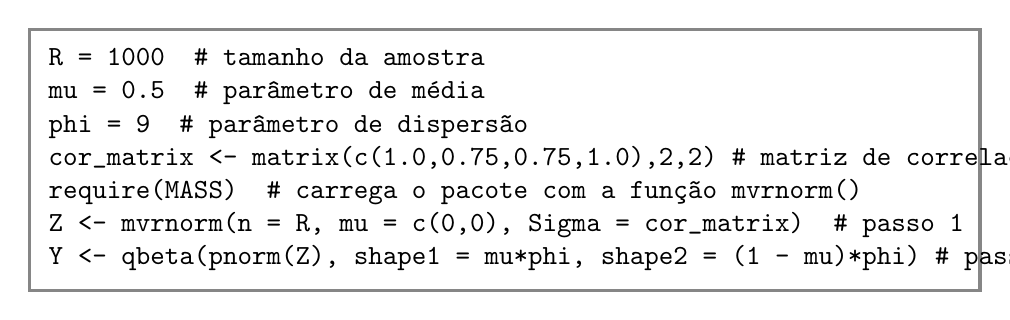
\begin{tikzpicture}
      \node [mybox] (box){
        \begin{minipage}{0.955\textwidth}
\begin{verbatim}
R = 1000  # tamanho da amostra
mu = 0.5  # parâmetro de média
phi = 9  # parâmetro de dispersão
cor_matrix <- matrix(c(1.0,0.75,0.75,1.0),2,2) # matriz de correlação
require(MASS)  # carrega o pacote com a função mvrnorm()
Z <- mvrnorm(n = R, mu = c(0,0), Sigma = cor_matrix)  # passo 1
Y <- qbeta(pnorm(Z), shape1 = mu*phi, shape2 = (1 - mu)*phi) # passo 2
\end{verbatim}
        \end{minipage}
      };
    \end{tikzpicture}
  \end{program}
  \vspace{-0.5cm}
  \begin{footnotesize}
    \centering
    FONTE: O autor~(2018).
    \vspace{-0.28cm}
  \end{footnotesize}
  \label{fig:steps1e2}
\end{figure}

% ======================================================================
% ----------------------------------------------------------------------
\chapter{Modelo de regressão multivariado}
\label{cap:multivariatemodel}
% ======================================================================

Este Capítulo apresenta o novo modelo de regressão usado para análise de
variáveis respostas limitadas multivariada, o qual será chamado por
modelo de regressão quase-beta multivariado. A~\autoref{cap:modelo}
apresenta a estrutura do modelo, enquanto a~\autoref{cap:estimacao}
apresenta o método proposto para estimação dos parâmetros de regressão e
dispersão. Por fim, a~\autoref{cap:diagnostics} adapta técnicas de
diagnóstico para o modelo proposto.

\section{MODELO DE REGRESSÃO QUASE-BETA MULTIVARIADO}
\label{cap:modelo}

% END ==================================================================
% ----------------------------------------------------------------------
\chapter{Resultados}
\label{cap:resultados}
% Neste Capítulo são apresentados os resultados de três estudos de
% simulação, além da análise dos dados apresentados no
% \autoref{cap:aplicacoes}. O primeiro estudo de simulação foi conduzido
% para investigar o comportamento do algoritmo NORTA (NOR\textit{mal To
%   Anything}) na simulação de variáveis aleatórias beta correlacionadas
% (\autoref{cap:simul1}). O segundo visou checar propriedades dos
% estimadores para os parâmetros de dispersão, no contexto de análise de
% dados longitudinais (\autoref{cap:simulLong}). E o terceiro foi
% delineado para explorar a flexibilidade dos estimadores para lidar com
% múltiplas respostas correlacionadas (\autoref{cap:simul2}). Por fim, a
% \autoref{cap:resultIQA} apresenta os resultados da análise dos dados
% referente ao índice de qualidade da água (IQA), enquanto a
% \autoref{cap:resultcorporal} apresenta os resultados correpondentes ao
% percentual de gordura corporal.

% \section{ESTUDOS DE SIMULAÇÃO}

% \subsection{Comportamento do algoritmo NORTA}
% \label{cap:simul1}

% \begin{figure}[H]
%   \vspace{0.4cm}
%   \caption{VALORES MÍNIMOS E MÁXIMOS PARA A CORRELAÇÃO ENTRE DUAS
%     VARIÁVEIS ALEATÓRIAS BETA EM FUNÇÃO DAS MÉDIAS MARGINAIS E
%     DIFERENTES VALORES DO PARÂMETRO $\phi$}
%   \setlength{\abovecaptionskip}{.0001pt}
%   \vspace{-0.38cm}
%   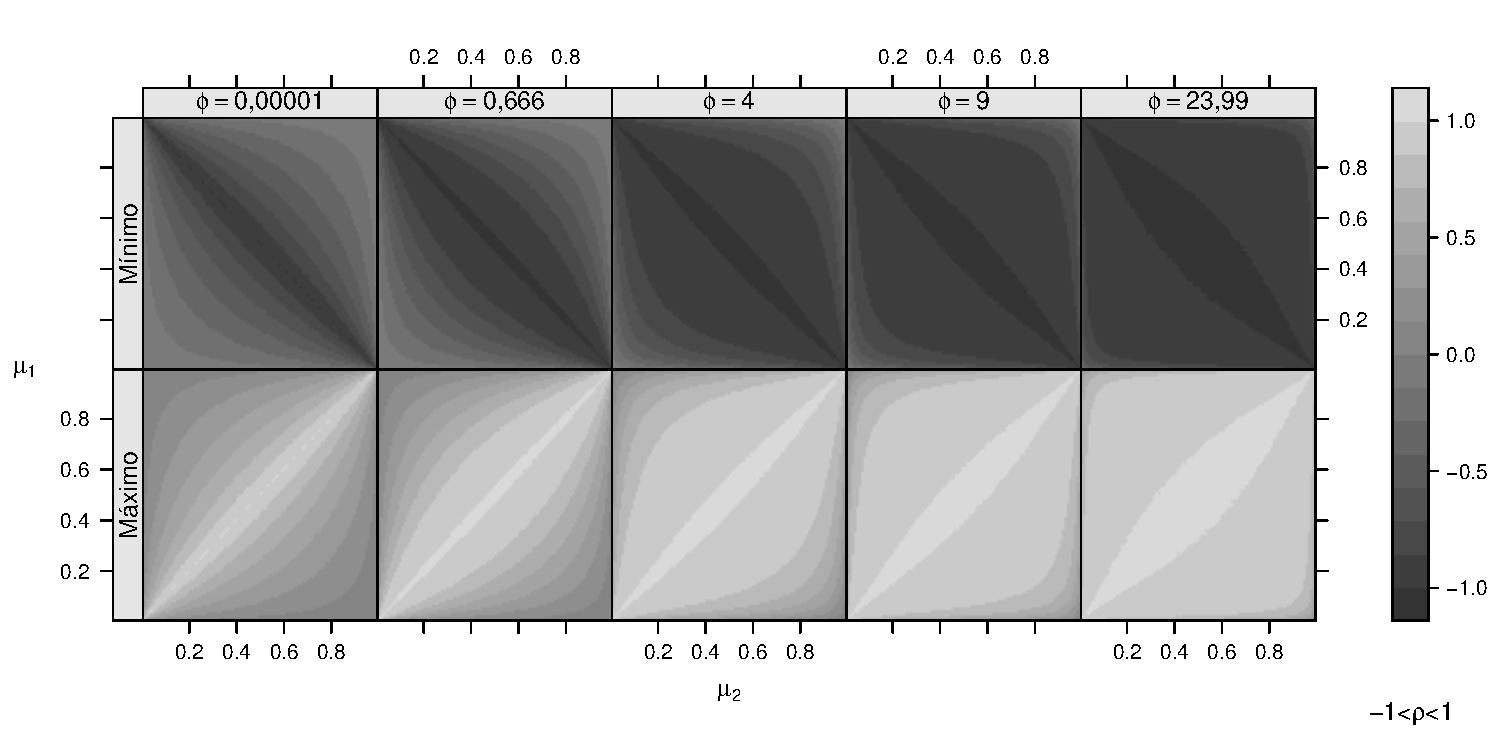
\includegraphics[width=16.0cm,height=7.6cm]{Figure10.pdf}
%   \vspace{-0.7cm}
%   \begin{footnotesize}
%     \centering
%     FONTE: O autor~(2018).
%     \vspace{0.15cm}
%   \end{footnotesize}
%   \label{fig:simulnorta}
% \end{figure}

% \begin{equation}
%   \label{eq:linearPredIQA}
%   g(\mu_{jki}) = \beta_0  + \beta_{1j}~\texttt{local}_{ji} + \beta_{2k}~\texttt{trimestre}_{ki},
% \end{equation}
% \noindent
% Na sequência, ajustou-se o modelo de regressão quase-beta multivariado
% aos dados do IQA, considerando as quatro estruturas acima mencionadas
% além de especificar a função de ligação \textit{logit} para o preditor
% linear~(\autoref{eq:linearPredIQA}).

% END ==================================================================
% ----------------------------------------------------------------------
\chapter{Considerações finais}
\label{cap:considefinais}
% O objetivo geral desta dissertação foi propor um novo modelo de
% regressão para análise de variáveis respostas limitadas multivariada. O
% modelo foi especificado usando apenas suposições de primeiro e segundo
% momentos. Para estimação dos parâmetros, adotou-se uma abordagem que
% combina as funções de estimação quase-score e Pearson para estimação dos
% parâmetros de regressão e dispersão, respectivamente. Assim, o modelo
% proposto nesta dissertação segue o estilo de quase-verossimilhança
% apresentado, onde a especificação do modelo é feita pela combinação da
% função de variância da distribuição binomial com as tradicionais funções
% de ligação para dados binários.

\section{FUTURE WORKS}

% END ==================================================================
% ----------------------------------------------------------------------
\setlength{\afterchapskip}{\baselineskip}
% ----------------------------------------------------------------------
\bibliography{referencias}
% ----------------------------------------------------------------------
\postextual
% ----------------------------------------------------------------------
% \begin{apendicesenv}
% \partapendices
% \addcontentsline{toc}{chapter}{\hspace{2.105cm}APPENDIX}
% \renewcommand{\ABNTEXchapterfontsize}{\ABNTEXsectionfont}
% \end{apendicesenv}
% ----------------------------------------------------------------------
% \begin{anexosenv}
% \partanexos
% \addcontentsline{toc}{chapter}{\hspace{2.105cm}ANNEX}
% \renewcommand{\ABNTEXchapterfontsize}{\ABNTEXsectionfont}
% \end{anexosenv}
%-----------------------------------------------------------------------
\phantompart
\printindex
%-----------------------------------------------------------------------
\end{document}
% END ==================================================================